%  ========================================================================
%  Copyright (c) 1985 The University of Washington
%
%  Licensed under the Apache License, Version 2.0 (the "License");
%  you may not use this file except in compliance with the License.
%  You may obtain a copy of the License at
%
%      http://www.apache.org/licenses/LICENSE-2.0
%
%  Unless required by applicable law or agreed to in writing, software
%  distributed under the License is distributed on an "AS IS" BASIS,
%  WITHOUT WARRANTIES OR CONDITIONS OF ANY KIND, either express or implied.
%  See the License for the specific language governing permissions and
%  limitations under the License.
%  ========================================================================
%

% Documentation for University of Washington thesis LaTeX document class
% by Jim Fox
% fox@washington.edu
%
%    Revised 2020/02/24, added \caption()[]{} option.  No ToC.
%
%    Revised for version 2015/03/03 of uwthesis.cls
%    Revised, 2016/11/22, for cleanup of sample copyright and title pages
%
%    This document is contained in a single file ONLY because
%    I wanted to be able to distribute it easily.  A real thesis ought
%    to be contained on many files (e.g., one for each chapter, at least).
%
%    To help you identify the files and sections in this large file
%    I use the string '==========' to identify new files.
%
%    To help you ignore the unusual things I do with this sample document
%    I try to use the notation
%       
%    % --- sample stuff only -----
%    special stuff for my document, but you don't need it in your thesis
%    % --- end-of-sample-stuff ---


%    Printed in twoside style now that that's allowed
%
 
\documentclass [11pt, proquest] {uwthesis}[2020/02/24]

\usepackage{graphicx}
 
%
% The following line would print the thesis in a postscript font 

% \usepackage{natbib}
% \def\bibpreamble{\protect\addcontentsline{toc}{chapter}{Bibliography}}

\setcounter{tocdepth}{1}  % Print the chapter and sections to the toc
 

% ==========   Local defs and mods
%

% --- sample stuff only -----
% These format the sample code in this document

\usepackage{alltt}  % 
\newenvironment{demo}
  {\begin{alltt}\leftskip3em
     \def\\{\ttfamily\char`\\}%
     \def\{{\ttfamily\char`\{}%
     \def\}{\ttfamily\char`\}}}
  {\end{alltt}}
 
% metafont font.  If logo not available, use the second form
%
% \font\mffont=logosl10 scaled\magstep1
\let\mffont=\sf
% --- end-of-sample-stuff ---
 



\begin{document}
 
% ==========   Preliminary pages
%
% ( revised 2012 for electronic submission )
%

\prelimpages
 
%
% ----- copyright and title pages
%
\Title{Planetesimal Accretion Beyond the Solar System: An Application to Systems of Tightly-Packed Inner Planets}
\Author{Spencer Wallace}
\Year{2023}
\Program{Astronomy}

\Chair{Thomas Quinn}{Chair}{Department of Chair}
\Signature{Rory Barnes}
\Signature{Eric Agol}

\copyrightpage

\titlepage  

 
%
% ----- signature and quoteslip are gone
%

%
% ----- abstract
%


\setcounter{page}{-1}
\abstract{%
This sample dissertation is an aid to students who are attempting
to format their theses with \LaTeX, a sophisticated
text formatter widely used by mathematicians and scientists everywhere.
 
\begin{itemize}
\item It describes the use of a specialized
macro package developed specifically for thesis production
at the University.
The macros customize \LaTeX\ for the correct thesis style,
allowing the student to concentrate on the substance of
his or her text.%
\footnote{See Appendix A to obtain the source to this
 thesis and the class file.}
\item It demonstrates the solutions to a variety of
formatting challenges found in thesis production.
\item It serves as a template for a real dissertation.
\end{itemize}
}
 
%
% ----- contents & etc.
%
\tableofcontents
\listoffigures
%\listoftables  % I have no tables

 
%
% ----- acknowledgments
%
\acknowledgments{% \vskip2pc
  % {\narrower\noindent
  The author wishes to express sincere appreciation to
  University of Washington, where he has had the opportunity
  to work with the \TeX\ formatting system,
  and to the author of \TeX, Donald Knuth, {\it il miglior fabbro}.
  % \par}
}

%
% ----- dedication
%
\dedication{\begin{center}to my dear wife, Joanna\end{center}}

%
% end of the preliminary pages
 
 
 
%
% ==========      Text pages
%

\textpages
 
\chapter {Introduction}

\chapter {Formation of Planetary Embryos in the Inner Solar System}

\section{Introduction} \label{sec:intro}

The standard scenario of terrestrial planet formation involves the pairwise accretion of small rocky bodies, called planetesimals, 
that condense from dust out of the protostellar disc \cite{safronov69}. This accretion process can be broken into a series of 
distinct stages. First, dust particles settle toward the midplane of the disc and clump together via gravitational instability 
\cite{goldreich73, youdin02}, streaming instabilities \cite{johansen07, johansen15}, turbulent concentration 
\cite{chambers10, cuzzi08, cuzzi10, hopkins16} or direct sticking \cite{okuzumi12, windmark12, garaud13, katoka13}. These 
formation models predict a wide variation in the initial size of planetesimals, ranging from hundreds of meters up to a few 
hundred kilometers in diameter.

After this condensation process ends, growth continues via pairwise collisions between planetesimals. Above about 1 km in size, 
gravitational focusing becomes effective and the collision rate strongly increases. This marks the beginning of the intermediate 
stage of accretion. During this phase, runaway growth \cite{duncan89, kokubo96, barnes09} quickly increases the size of the 
largest bodies. Eventually, the largest bodies grow massive enough to heat the small planetesimals, which then inhibits the 
runaway growth effect. This marks the transition into the phase of oligarchic growth in which the handful of large bodies all tend 
to grow at the same rate. This produces a bimodal size distribution of planetesimals, with many small bodies and a handful of 
very large bodies. During this phase, a combination of scattering events between the oligarchs and dynamical friction from the 
small planetesimals places the oligarchs on nearly circular orbits that are spaced apart by approximately 5-10 Hill radii 
\cite{kokubo98}. Eventually, the oligarchs accrete most of the available material in the vicinity of their orbit, which eventually 
throttles their growth rate. On much longer time scales, the large bodies perturb each other onto crossing orbits, forming Mars to 
Earth sized bodies via occasional collisions. This phase of late stage accretion is highly chaotic and takes much longer to play 
out than the previous stages \cite{chambers98, raymond06}.

Generally, planetesimal accretion models fail to produce a configuration of planets that resembles that of the Solar System. 
Planets produced in the vicinity of Mars are systematically too massive \cite{wetherill92, raymond09, morishima10, izidoro15} 
and the terrestrial planets that form are too eccentric compared to their Solar System counterparts 
\cite{chambers98, agnor99, chambers01}. In addition, the present day water content of Earth, along with the large D/H ratio of 
Venus \cite{donahue82} does not match with models of solids that condensed out of the Solar nebula at 1 AU.

These issues all have proposed solutions, which generally involve altering the initial conditions for late-stage
accretion simulations. The condition of the Solar System at the beginning of the late stage accretion phase is poorly constrained. 
This is mostly due to the fact that planetesimal formation, and therefore the intermediate accretion phase which produces the 
planetary embryos, is not well understood. Although the present day population of small Solar System bodies has continued to 
evolve since the end of the intermediate accretion phase, the current size frequency distribution (SFD) of asteroid belt and 
Kuiper belt objects contains some clues about the accretion history. \cite{morbidelli09} argued that the SFD of asteroid belt 
objects larger than 100 km in diameter has been largely unchanged, aside from a size independent depletion factor. 
\cite{duncan89} did a long term stability analysis of small Solar System objects and found that small bodies left over from 
accretion should still be largely unperturbed. For these reasons, it should be possible to connect observables in the Solar System to planetesimal formation theories by modeling only the intermediate stages of accretion.

There are two common ways to model planetesimal growth. A powerful approach is to use statistical methods to track the 
evolution of large groups of planetesimals. This is known as the particle-in-a-box method \cite{greenberg78, wetherill89}. The 
evolution of growth is followed by tracking planetesimals in discrete bins of mass and semi-major axis. This removes the need to 
calculate the motion of every individual body and allows very large collections of planetesimals to be followed. Unfortunately, the 
dynamics that governs the evolution of these bodies does not always naturally emerge with this approach. As an example, 
\cite{weidenschilling11} found that a careful treatment of three body encounters led to a different prediction for the initial size 
distribution of planetesimals near the asteroid belt. Additionally, the particle-in-a-box method is not well suited for studying 
oligarchic growth because the largest mass bins, which dominate the evolution in this stage, contain small numbers of bodies. 
Non-gravitational effects such as gas drag and fragmentation require extra care to implement self-consistently 
\cite{leinhardt08}, although it has been successfully done \cite{wetherill93, chambers01}. To alleviate some of these issues 
while still being able to model large populations, a newer hybrid approach, in which large bodies are treated as single entities 
and planetesimals are treated as statistical ensembles has been developed 
\cite{weidenschilling97, kenyon06, levison12, morishima15}.

The most reliable and straightforward approach is to use N-body methods to follow the evolution and growth of the planetesimals 
\cite{lecar86}. By tracking the individual motions of bodies, the dynamics governing their evolution naturally emerges, no matter 
what the distribution of bodies looks like. However, N-body simulations involving collision detection are extremely 
computationally expensive, which severely limits both the resolution and number of timesteps that can be achieved. This is why 
there are very few studies of runaway and oligarchic with direct N-body simulations in the literature 
\cite{kokubo96, kokubo98, kokubo02, barnes09}. Instead, N-body methods are most commonly used to study late stage 
accretion, where the self-gravity and collisional evolution of the residual planetesimals is largely unimportant 
\cite{chambers98, agnor99,  chambers01, obrien06, morbidelli09}.

To date, we are not aware of any N-body simulations that resolve both the runaway and oligarchic growth phase  with more than 
about $10^4$ particles. At this resolution, stochasticity likely has a significant influence on dynamical friction and resonances 
may not be sufficiently resolved. \cite{raymond06} found that insufficient planetesimal resolution during the oligarchic growth 
phase limits the effectiveness of dynamical friction felt by the oligarchs, producing a population of embryos with unrealistically 
high eccentricities. This idea has also been applied to planet migration through a disc of planetesimals. \cite{cionco02} showed 
that resonances make a significant contribution to the dynamical friction torque exerted by the disc on the planet. This 
phenomenon requires the planetesimals to be finely resolved \cite{brunini07}. Dynamical friction is also facilitated via 
resonances in galactic dynamics \cite{lyndenbell72}. \cite{weinberg07, weinberg07} examined the effect of N-body particle 
counts on galaxy dynamics and showed that resonant interactions between the bar and halo were only effective with sufficient 
particle phase space coverage.

For these reasons, we motivate the need for a high resolution N-body simulation of planetesimal growth. We do this to better 
understand the effect that dynamical friction has on the intermediate stages of terrestrial planet growth and to examine what 
predictions a high resolution model makes about the residual population of planetesimals in the Solar System. In particular, 
resonances which are only effective with fine enough resolution, may have an important influence on planetesimal growth. In this 
paper, we investigate planetesimal evolution during the runaway and oligarchic growth phases with a direct N-body model. We 
begin by simulating an annulus of planetesimals with similar resolution to \cite{kokubo98} to validate our model. We then run the 
same configuration with 100x more particles to better understand the effects of resolution on the intermediate stages of 
terrestrial planet growth.

In section \ref{sec:sim}, we describe the simulation code that we use and provide a detailed description of the collision model. 
We also summarize the initial conditions used. In section \ref{sec:results}, we present the results of the low and high resolution 
simulation of terrestrial planet growth and highlight differences between the two. We find that a bump develops in the mass 
distribution of the high resolution simulation, which does not appear in the low resolution run. This feature manifests itself shortly 
after oligarchic growth commences and we infer that it is produced by extra heating via mean motion resonances between the 
oligarchs and small planetesimals. To further demonstrate this effect, we re-run the high resolution simulation with a narrower 
annulus (depopulating many of the resonances) and show that this reduces the prominence of the bump in the mass distribution. 
In section \ref{sec:dynfric}, we present a set of collisionless simulations of a planetary embryo embedded in an annulus of 
planetesimals. This more clearly demonstrates the differences in dynamical behavior between the low and high resolution 
models. In section \ref{sec:intermed}, we present two more simulations of planetesimal growth at intermediate resolutions and 
demonstrate that the location of the bump is sensitive to the initial planetesimal mass. Finally, section \ref{sec:discussion} 
connects these new results to our present understanding of terrestrial planet growth and we discuss the additional steps 
necessary to use our results to constrain the initial size of planetesimals in the Solar System.

\section{Simulations} \label{sec:sim}

\subsection{Numerical Methods} \label{sec:numerical}

All of the simulations described in this paper were performed with the highly parallel N-body code {\sc ChaNGa} . 
{\sc ChaNGa} is written in the {\sc CHARM++} programming language and has been shown to perform well when using up to 
half a million processors \cite{menon15} simultaneously. Gravitational forces are calculated using a modified Barnes-Hut tree 
algorithm with hexadecapole order expansions of the moments. For all of the simulations described in this paper, a node 
opening criterion of $\Theta_{BH}$ = 0.7 was used. \cite{richardson00} was able to resolve mean motion resonances in a 
terrestrial disc using a similar tree code with the same node opening criterion, so we expect that our model should properly 
handle resonance effects as well. The equations of motion are integrated using a kick-drift-kick leapfrog scheme. For more 
information about the implementation of {\sc ChaNGa} see \cite{jetley08}.

\subsection{Collision Model} \label{sec:collModel}

{\sc ChaNGa} is a smoothed particle hydrodynamics code originally designed for cosmology simulations. In order to use 
{\sc ChaNGa} to study planetesimal coagulation, we implemented a hard-body collision model that treats particles as solid 
objects with a fixed radius, rather than as smooth tracers of a fluid with a characteristic softening length. This work was largely 
based off of the hard body collision implementation in {\sc pkdgrav}, which is described in \cite{richardson94} and 
\cite{richardson00}.

Collisions are predicted at the beginning of each drift step by extrapolating the positions of the particles forward using the 
velocities calculated during the first kick. For each particle, the closest 64 neighbors are considered in the collision search. 
Because {\sc ChaNGa} is a tree code, the nearest neighbors of a particle can be retrieved in $\mathcal{O}(N\log{}N)$ time. After 
extrapolating the positions forward and checking for overlap with any neighbors, the earliest collision time $t_{coll}$ is stored for 
each particle.

After the prediction phase, particles with $t_{coll}$ less than the time step size $\Delta T$ must have their collisions resolved. For 
simplicity, all collisions in our simulations result in perfect accretion. \cite{ida93} showed that excluding the effects of 
fragmentation and collisional rebound does not qualitatively change the growth modes of the planetesimals. A merger between 
two particles of mass $m_{1}$ and $m_{2}$ results in a single particle of mass $M = m_{1} + m_{2}$, with the radius set to 
conserve density. The position and velocity of the resulting particle is set to the centre of mass position and velocity of the 
colliders at the moment of contact. The resulting merged particle is then drifted to the end of the step. If multiple collisions are 
predicted during a time step, the earliest collision is resolved first. Because resolving a collision can result in another imminent 
collision, collisions must be resolved one by one, with a new prediction check being run each time.

As in \cite{kokubo96, kokubo98} we accelerate the accretion process by artificially inflating the physical radius of the bodies by 
a factor of $f$. This technique reduces the accretion time-scale by approximately a factor of $f^{2}$, significantly reducing the 
number of timesteps that must be integrated. Additionally, inflating the particle radii allows us to use a smaller annulus with less 
planetesimals. The reason we cannot use an arbitrarily skinny annulus is because the edges tend to expand outward due to the 
unrealistic boundary conditions, decreasing the surface density. The time-scale for this expansion is set by the two body 
relaxation time-scale, which scales with $N$. Reducing the accretion time-scale by increasing $f$ allows us to study 
planetesimal growth with a smaller, less computationally expensive annulus.

We must be careful, however, to choose a value of $f$ that is not too large. The rms eccentricity and inclination of the 
planetesimal disc grows as gravitational encounters transform energy due to Keplerian shear into random motions. By 
accelerating the growth rate, we cause the transitions between growth modes to happen early, when the disc is less dynamically 
excited. This discrepancy is partly compensated for by the fact that our model ignores the effects of gas drag, which would damp 
the eccentricities and inclinations of the planetesimals. We adopt $f=6$ for our calculations, which reduces the amount of 
gravitational scattering by less than 10\% of its true value and does not qualitatively change the modes of planetesimal growth 
\cite{kokubo98}.

\noindent As previously mentioned, simulation (ii) is meant to be compared with the results of \cite{kokubo98}. This allows us to 
both validate our collision model and also have a baseline to compare our simulations to. In both cases, the planetesimals are 
distributed randomly in an annulus centred at 1 AU with a width $\Delta a = 0.085$ AU around a 1 $\mathrm{M_{\odot}}$ star. 
This annulus width was chosen so that the required particle count is minimized without boundary effects influencing planetesimal 
growth. The surface mass density of the ring is set to 10 g cm$^{-2}$, which approximately corresponds to the minimum-mass 
solar nebula model \cite{hayashi81} at 1 AU. In case (i), the eccentricities and inclinations are taken from a Rayleigh distribution 
\cite{ida92} with $\langle e^2 \rangle^{1/2} = 2 \langle i^2 \rangle^{1/2} = 4 h/a$, where $h$ is the mutual Hill radius. To match 
the same eccentricity and inclination dispersion with larger planetesimals in case (ii), we use $\langle e^2 \rangle^{1/2} = 2 
\langle i^2 \rangle^{1/2} = 0.635 h/a$. In both simulations, the planetesimals are given an internal density of 2 g cm$^{-3}$. We 
use fixed timesteps with $\Delta T$ = 0.0025 years and evolve the simulations for 20,000 years. Large timesteps diminish the 
effectiveness of gravitational focusing, which inhibits the collision rate. We find that the collision rate is converged below $\Delta 
T$ = 0.0025 years. The integration time was chosen to be comparable to the orbital repulsion and Hill radius growth time-scale 
\cite{kokubo95} so that the effects of oligarchic growth are fully realized by the end of the simulation.

It is worth noting that simulation (i) was a very computationally expensive undertaking. In total, the full 20,000 years of 
integration required approximately 130,000 CPU hours and over 50 days of wall clock time.

\begin{figure}
    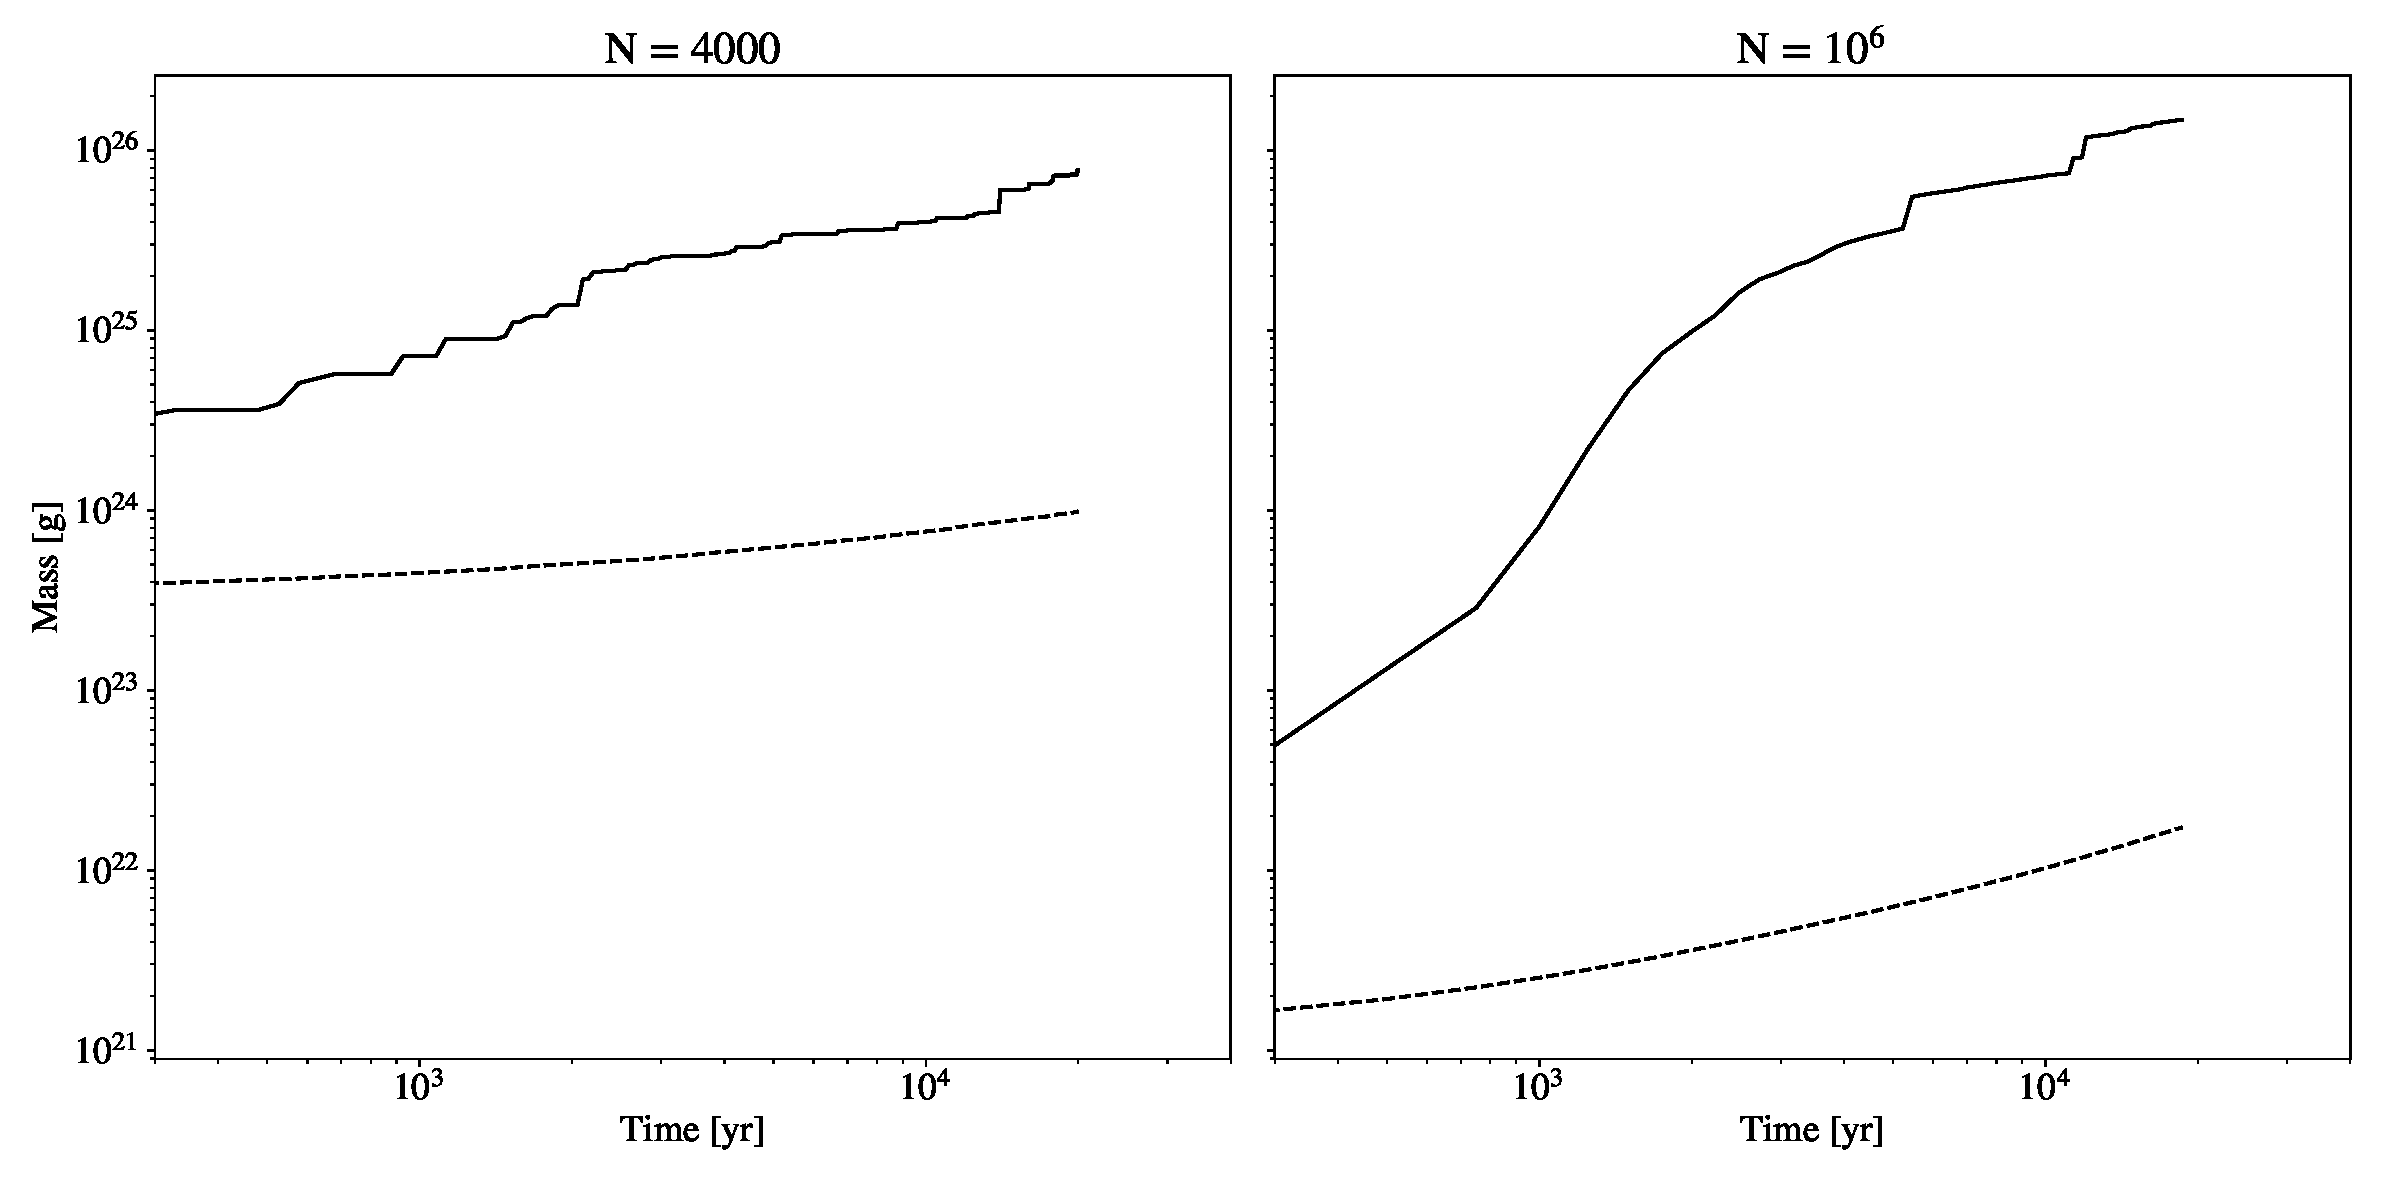
\includegraphics[width=\textwidth]{figures/plSS/mass_evo.eps}
    \caption{Evolution of the maximum (solid curve) and mean (dashed curve) planetesimal mass in the N=4000 and N=$10^6$ particle simulations. At early times, the maximum mass grows more quickly than the mean mass, which is indicative of runaway growth. After a few thousand years, the separation between the curves becomes a constant factor, signalling the start of oligarchic growth.
    \label{fig:mass_evo}}
\end{figure}

\begin{figure}
    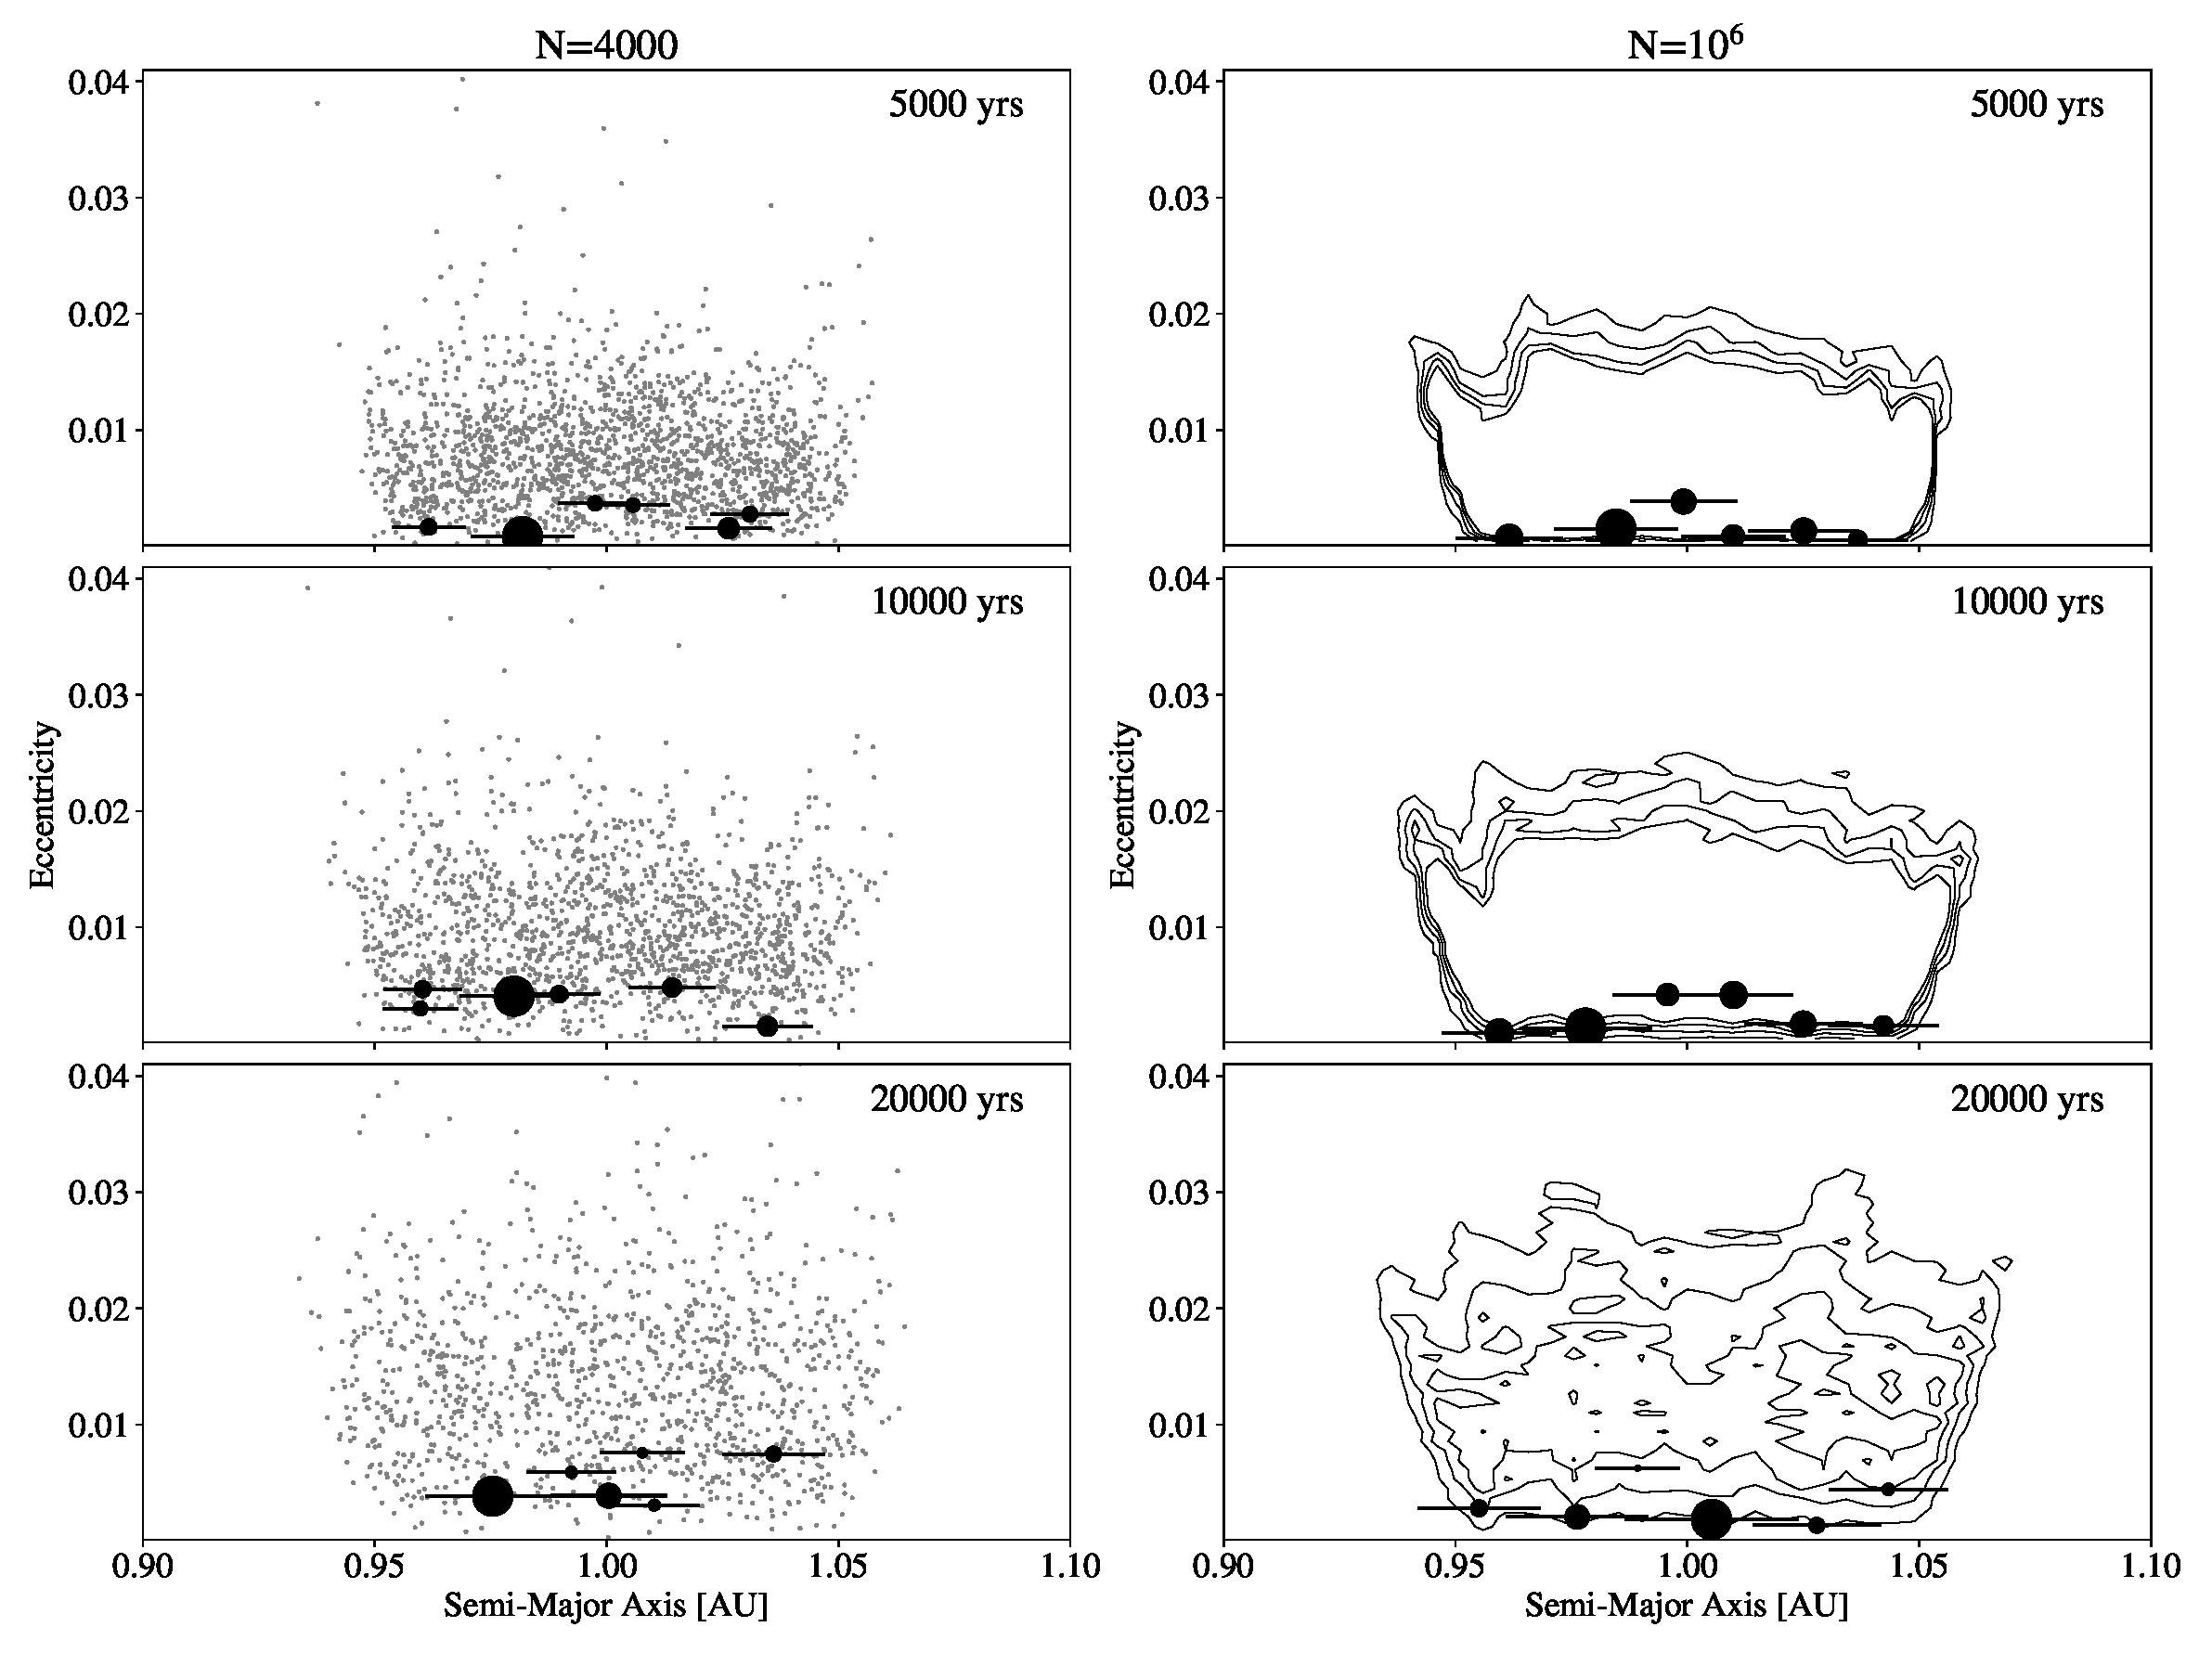
\includegraphics[width=\textwidth]{figures/plSS/ecc_evo.eps}
    \caption{Snapshots from the low and high resolution models in the $a-e$ plane. On the left, the light dots represent individual planetesimals, while the contours on the right hand plots represent curves of constant number density. The contour levels are the same between all panels and correspond to $7.8 \times 10^6$, $1.6 \times 10^7$, $2.3 \times 10^7$, and $3.1 \times 10^7$ planetesimals per AU per unit eccentricity. The black circles denote the configuration of the 6 largest bodies in the simulation, with the area of the circles scaled to the mass of the body. The horizontal error bars are scaled to 5 times the Hill radius of the bodies.
    \label{fig:ae}}
\end{figure}

\begin{figure}
    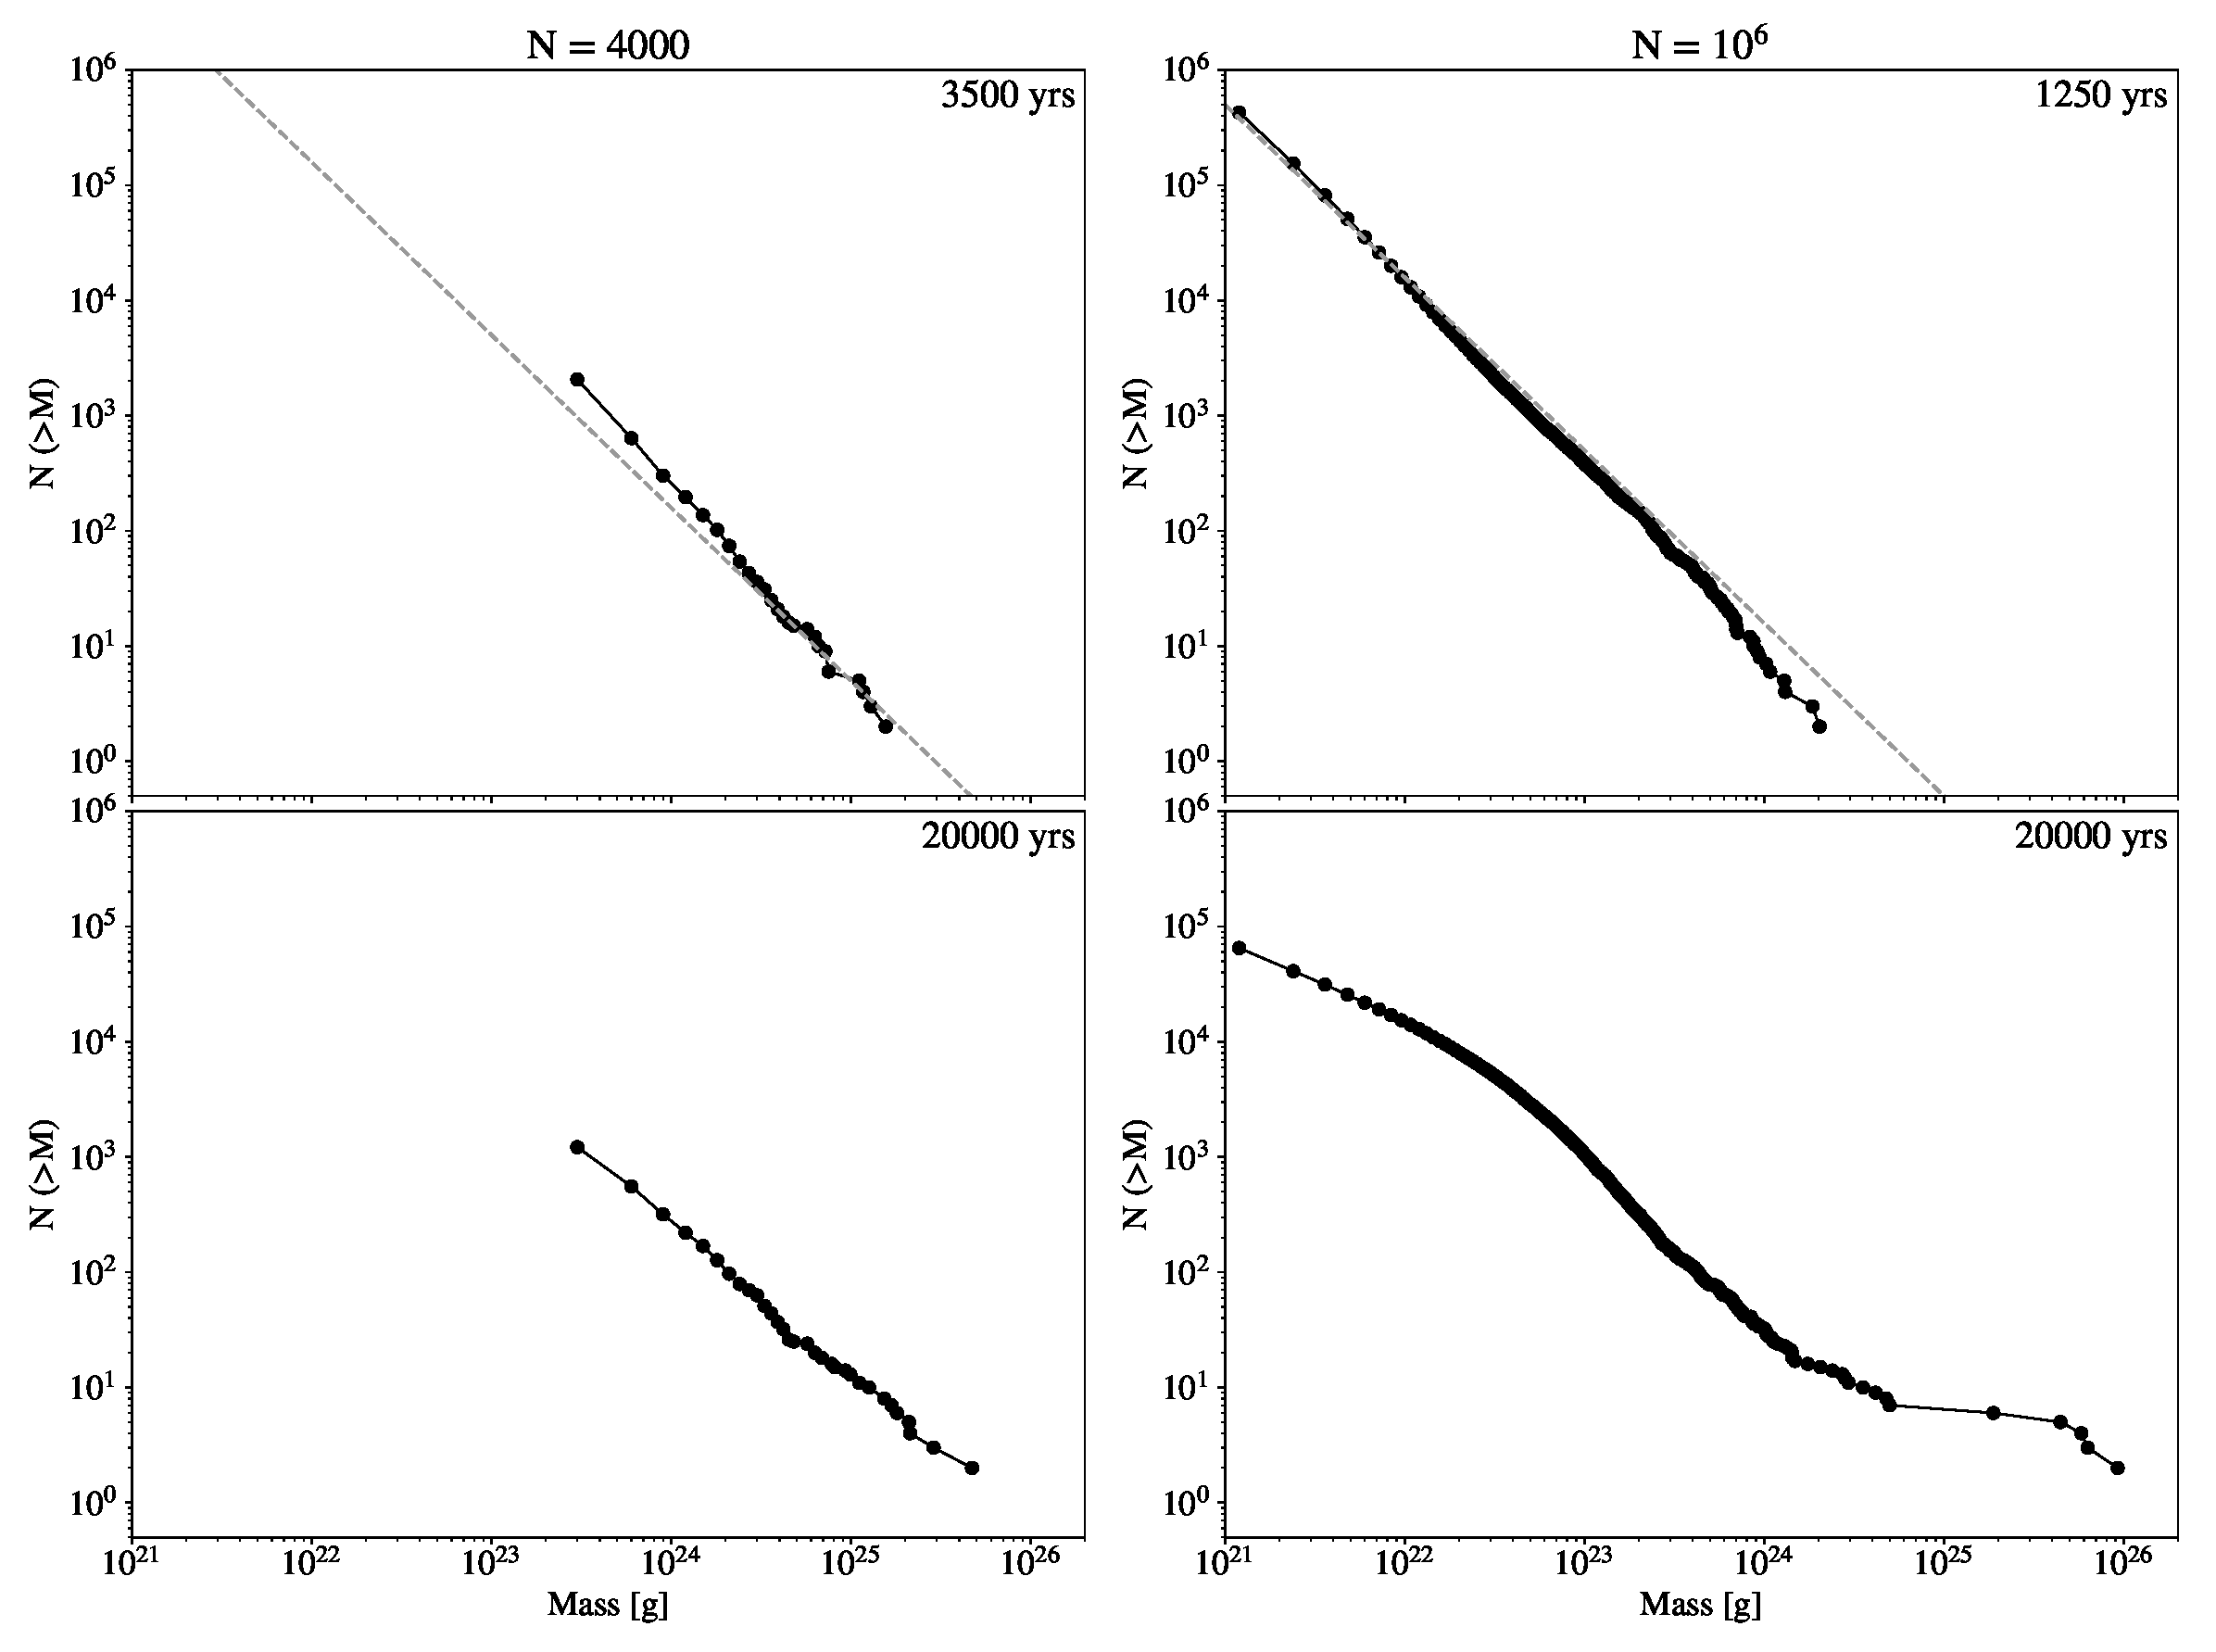
\includegraphics[width=\textwidth]{figures/plSS/mass_spectrum_evo.eps}
    \caption{Cumulative number of bodies in each mass bin for the low and high resolution runs, shown at the end of runaway growth (top row) and the end of the simulation (bottom row). The dashed line indicates a slope of -1.5, which is characteristic of runaway growth.
    \label{fig:mass_spectrum_evo}}
\end{figure}

\subsection{Initial Conditions} \label{sec:ics}

We begin by using our collision model to perform two sets of calculations:

(i) $10^{6}$ equal mass bodies with $m = 1.2 \times 10^{21}$ g

(ii) 4000 equal mass bodies with $m = 3 \times 10^{23}$ g

\section{Results} \label{sec:results}

\subsection{Low vs High Resolution}\label{sec:lowvshigh}

We begin by comparing the evolution of growth between the low resolution (N=4000) and high resolution (N=$10^{6}$) models. 
As planetesimals collide and grow, gravitational focusing becomes increasingly effective and the relative growth rate increases 
with mass \cite{greenberg78}. Figure \ref{fig:mass_evo} shows the evolution of the average and maximum planetesimal 
mass in both simulations. Runaway growth at early times is evident from the fact that the maximum mass grows more quickly 
than the mean mass. Eventually, the largest bodies begin to dynamically heat the neighboring planetesimals, which slows the 
growth rate of the largest bodies.

\chapter {Detecting Cold Jupiters via Collisional Grinding of Planetesimals}

\chapter {Formation of Planetary Embryos at Short Orbital Periods}

\chapter {In-Situ Formation of STIPs}

%
% ==========   Bibliography
%
\nocite{*}   % include everything in the uwthesis.bib file
\bibliographystyle{plain}
\bibliography{uwthesis}
%
% ==========   Appendices
%
\appendix
\raggedbottom\sloppy
 
% ========== Appendix A
 
\chapter{Where to find the files}
 
The uwthesis class file, {\tt uwthesis.cls}, contains the parameter settings,
macro definitions, and other \TeX nical commands which
allow \LaTeX\ to format a thesis.  
The source to
the document you are reading, {\tt uwthesis.tex},
contains many formatting examples
which you may find useful.
The bibliography database, {\tt uwthesis.bib}, contains instructions
to BibTeX to create and format the bibliography.
You can find the latest of these files on:

\begin{itemize}
\item My page.
\begin{description}
\item[] \verb%https://staff.washington.edu/fox/tex/thesis.shtml%
\end{description}

\item CTAN
\begin{description}
\item[]  \verb%http://tug.ctan.org/tex-archive/macros/latex/contrib/uwthesis/%
\item[]  (not always as up-to-date as my site)
\end{description}

\end{itemize}

\vita{Jim Fox is a Software Engineer with IT Infrastructure Division at the University of Washington.
His duties do not include maintaining this package.  That is rather
an avocation which he enjoys as time and circumstance allow.

He welcomes your comments to {\tt fox@uw.edu}.
}


\end{document}
